% Mammography problem from 'Intro to Bayes'
% Author: John Henderson
\documentclass[10pt]{article}
\usepackage{tikz}
%%%<
\usepackage{verbatim}
%\usepackage[active,tightpage]{preview}
%\PreviewEnvironment{tikzpicture}
%\setlength\PreviewBorder{5pt}%
%%%>
\begin{comment}
:Title: Mammography problem from 'Intro to Bayes'
:Tags: Nodes and Shapes;Node positioning;Text and math;Diagrams;Mathematics
:Author: John Henderson
:Slug: bayes

The following was created in response to reading about "the mammography
problem," a commonly used example illustrating the use of Bayesian
Probability, on Eliezer Yudkowsky's page, "An Intuitive Explanation of
Bayes' Theorem." The visualization presents the problem as involving
"sieves" which behave differently depending on whether the individual
passing through has or does not have cancer, illustrating the split
probability created by the reliability of a mammography (chance of
producing true positives and false positives). The illustration was posted
on LessWrong.com, a site devoted to rationality, created by Yudkowsky.
\end{comment}
\usetikzlibrary{positioning,decorations.pathreplacing,shapes}
\usepackage[english]{babel}
\usepackage{microtype}
\usepackage[hmargin=1.5cm,vmargin=1cm]{geometry}
\usepackage{amsmath}
\DeclareMathOperator{\p}{p}
\newcommand*{\cancer}{\text{cancer}}
\newcommand*{\testp}{\text{test}+}
\begin{document}
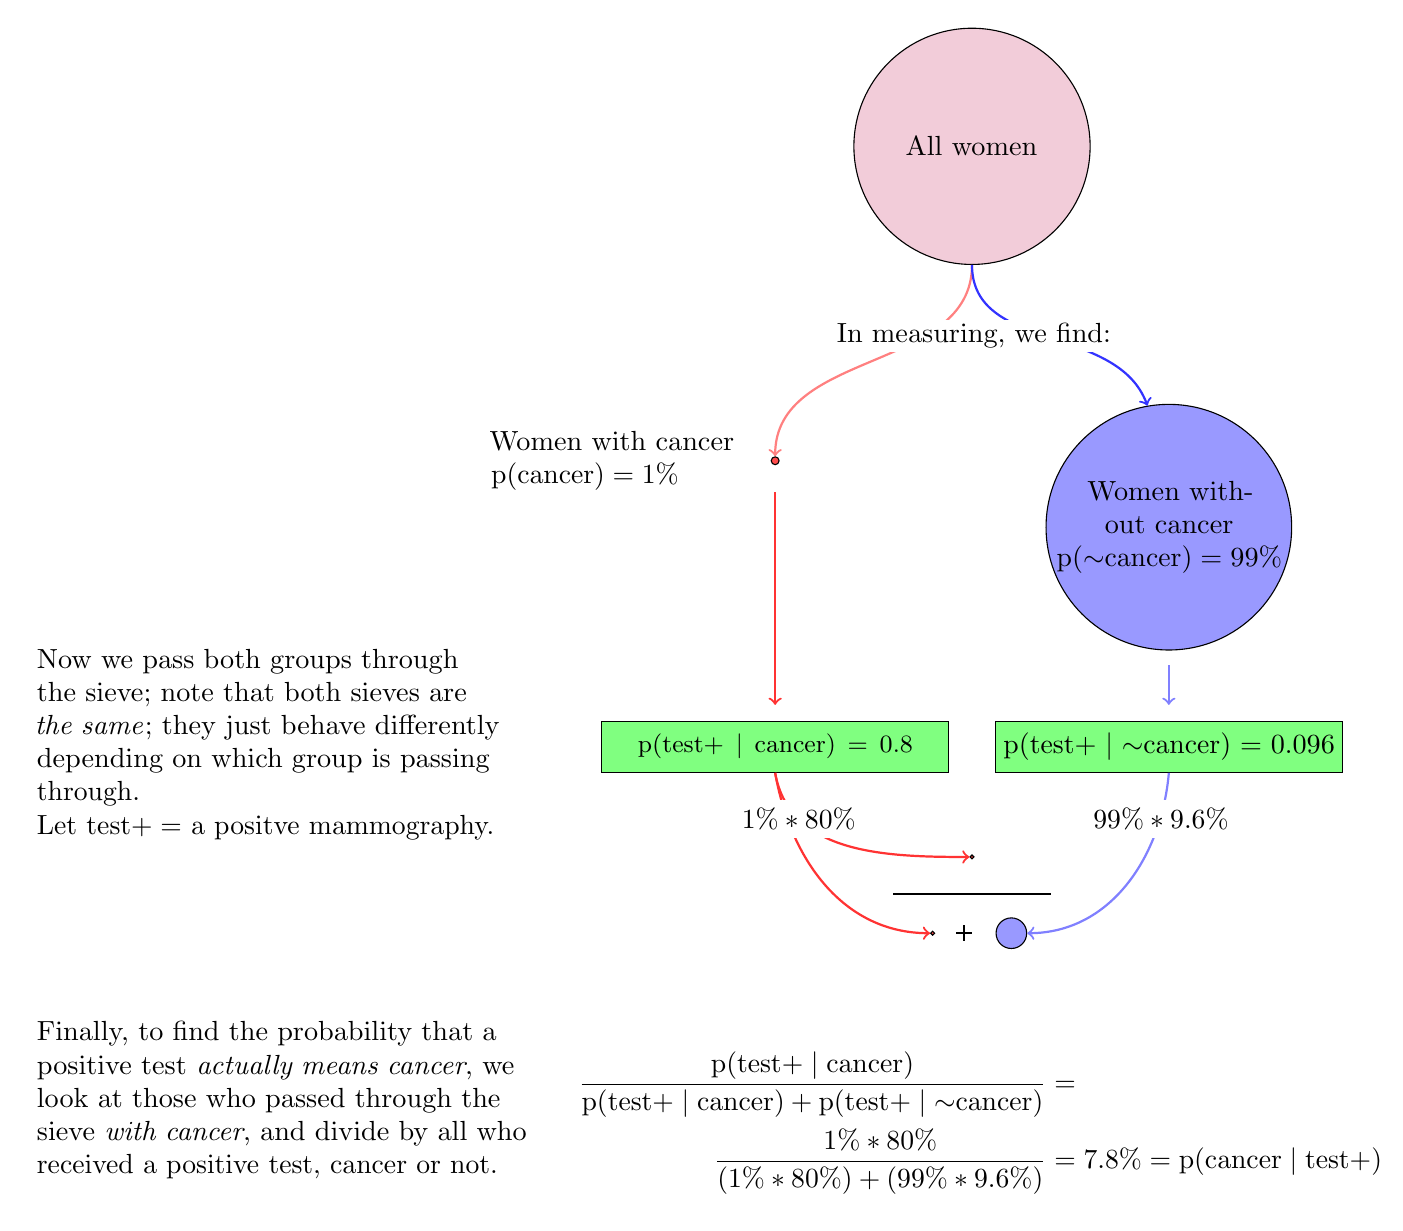
\begin{tikzpicture}[%
  % common options for blocks:
  block/.style = {draw, fill=blue!30, align=center, anchor=west,
              minimum height=0.65cm, inner sep=0},
  % common options for the circles:
  ball/.style = {circle, draw, align=center, anchor=north, inner sep=0}]

% circle illustrating all women
\node[ball,text width=3cm,fill=purple!20] (all) at (6,0) {All women};

% two circles showing split of p{cancer} and p{~cancer}
\node[ball,fill=red!70,text width=0.1cm,anchor=base] (pcan) at (3.5,-5.5) {};
\node[ball,fill=blue!40,text width=2.9cm,anchor=base] (pncan) at (8.5,-6)
   {Women without cancer\\
    $\p({\sim}\cancer) = 99\%$};

% arrows showing split from all women to cancer and ~cancer
\draw[->,thick,draw=red!50] (all.south) to [out=270,in=90] (pcan.north);
\draw[->,thick,draw=blue!80] (all.south) to [out=270,in=110] (pncan.100);

% transition from all women to actual cancer rates
\node[anchor=north,text width=10cm,inner sep=.05cm,align=center,fill=white]
  (why1) at (6,-3.7) {In measuring, we find:};

% note illustration the p{cancer} circle (text won't fit inside)
\node[inner sep=0,anchor=east,text width=3.3cm] (note1) at (3.2,-5.5) {
   Women with cancer $\p(\cancer) = 1\%$};

% draw the sieves
\node[block,anchor=north,text width=4.4cm,fill=green!50] (tray1) at
   (3.5,-8.8) {\small{$\p(\testp\mid\cancer)=0.8$}};

\node[block,anchor=north,text width=4.4cm,fill=green!50] (tray2) at
   (8.5,-8.8) {$\p(\testp\mid{\sim}\cancer)=0.096$};

% text explaining how p{cancer} and p{~cancer} behave as they
% pass through the sieves
\node[anchor=west,text width=6cm] (note1) at (-6,-9.1) {
   Now we pass both groups through the sieve; note that both
     sieves are \emph{the same}; they just behave differently
     depending on which group is passing through. \\ 
     Let $\testp=$ a positve mammography.};

% arrows showing the circles passing through the seives
\draw[->,thick,draw=red!80] (3.5,-5.9) -- (3.5,-8.6);
\draw[->,thick,draw=blue!50] (8.5,-8.1) -- (8.5,-8.6);

% numerator
\node[ball,text width=0.05cm,fill=red!70] (can) at (6,-10.5) {};

% dividing line
\draw[thick] (5,-11) -- (7,-11);

% demoniator
\node[ball,text width=0.39cm,fill=blue!40,anchor=base] (ncan) at (6.5,-11.5) {};
\node[ball,text width=0.05cm,fill=red!70,anchor=base] (can2) at (5.5,-11.5) {};

% plus sign in denominator
\draw[thick] (5.9,-11.4) -- (5.9,-11.6);
\draw[thick] (5.8,-11.5) -- (6,-11.5);

% arrows showing the output of the sieves formed the fraction
\draw[->,thick,draw=red!80] (tray1.south) to [out=280,in=180] (can);
\draw[->,thick,draw=red!80] (tray1.south) to [out=280,in=180] (can2);
\node[anchor=north,inner sep=.1cm,align=center,fill=white] (why2) at
   (3.8,-9.8) {$1\% * 80\%$};

\draw[->,thick,draw=blue!50] (tray2.south) to [out=265,in=0] (ncan);
\node[anchor=north,inner sep=.1cm,align=center,fill=white] (why2) at
   (8.4,-9.8) {$99\% * 9.6\%$};

% explanation of final formula
\node[anchor=north west,text width=6.5cm] (note2) at (-6,-12.5)
   {Finally, to find the probability that a positive test
       \emph{actually means cancer}, we look at those who passed
       through the sieve \emph{with cancer}, and divide by all who
       received a positive test, cancer or not.}; 

% illustrated fraction turned into math
\node[anchor=north,text width=10cm] (solution) at (6,-12.5) {
  \begin{align*}
      \frac{\p(\testp\mid\cancer)}{\p(\testp\mid\cancer)
        + \p(\testp\mid{\sim}\cancer)} &= \\
      \frac{1\% * 80\%}{(1\% * 80\%) + (99\% * 9.6\%)} &= 7.8\%
        = \p(\cancer\mid\testp)
   \end{align*}};
\end{tikzpicture}
\end{document}
